\documentclass[tikz,border=2pt]{standalone}
\usepackage{amsmath}
\usepackage{newtxtext,newtxmath} % Times-like to match IEEEtran
\usetikzlibrary{arrows.meta,positioning,calc,fit,shapes.multipart,decorations.pathmorphing}
\tikzset{>=Latex, line/.style={line width=0.8pt}, box/.style={draw, rounded corners=2pt, minimum width=28mm, minimum height=12mm, align=center},
note/.style={font=\footnotesize}}

\begin{document}
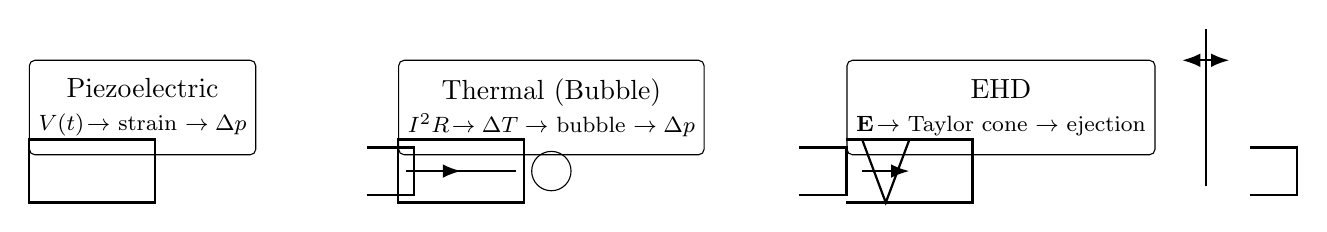
\begin{tikzpicture}[node distance=10mm]
% Boxes
\node[box] (piezo) {Piezoelectric\\ \footnotesize $V(t)\!\rightarrow$ strain $\rightarrow \Delta p$};
\node[box, right=18mm of piezo] (thermal) {Thermal (Bubble)\\ \footnotesize $I^2R\!\rightarrow \Delta T \rightarrow$ bubble $\rightarrow \Delta p$};
\node[box, right=18mm of thermal] (ehd) {EHD\\ \footnotesize $\mathbf{E}\!\rightarrow$ Taylor cone $\rightarrow$ ejection};

% Icons (minimal, monochrome)
\draw[line] ([yshift=-6mm]piezo.south west) rectangle ++(16mm,8mm); % cavity
\draw[line] ([xshift=14mm,yshift=-5mm]piezo.south east) -- ++(6mm,0) -- ++(0,6mm) -- ++(-6mm,0); % nozzle
\draw[->,line] ([xshift=20mm,yshift=-2mm]piezo.south east) -- ++(6mm,0);

\draw[line] ([yshift=-6mm]thermal.south west) rectangle ++(16mm,8mm); % chamber
\draw[line] ([xshift=1mm,yshift=-2mm]thermal.south west) -- ++(14mm,0);
\draw[line] ([xshift=12mm,yshift=-5mm]thermal.south east) -- ++(6mm,0) -- ++(0,6mm) -- ++(-6mm,0); % nozzle
\draw (thermal.south) ++(0,-2mm) circle (2.5mm); % bubble
\draw[->,line] ([xshift=20mm,yshift=-2mm]thermal.south east) -- ++(6mm,0);

\draw[line] ([yshift=-6mm]ehd.south west) -- ++(16mm,0) -- ++(0,8mm) -- ++(-16mm,0);
\draw[line] ([xshift=12mm,yshift=-5mm]ehd.south east) -- ++(6mm,0) -- ++(0,6mm) -- ++(-6mm,0); % nozzle
\draw[line] ([xshift=5mm,yshift=-6mm]ehd.south west) -- ++(3mm,8mm) -- ++(-6mm,0) -- cycle; % cone
\draw[line] ([xshift=26mm,yshift=-10mm]ehd.center) -- ++(0,20mm); % counter electrode
\draw[<->,line] ([xshift=23mm,yshift=6mm]ehd.center) -- ++(6mm,0);
\end{tikzpicture}
\end{document}
